\part{Construction du modèle}
    \chapter{Les principes généraux}
        \section{Contenu du texte d'une liste d'ingrédients}

        En général, chaque ingrédient sera présent une seule fois dans la liste (cf. section \mref{listes_ingredients})

        Le calcul d'embeddings via des modèles tels que SVD ou Word2Vec fait peu de sens.
        \newline
        \newline
        \emphbox{l'extraction des textes se fait au format \emph{Bag Of Words}, sans utiliser de notion d'IDF. L'utilsation de TF semble églament ne pas amener de valeur à priori.}

        \section{Limitation à l'identification des listes d'ingrédients}

        On est sur une taxonomie d'informations limitée dans les fiches techniques.

        On pourrait envisager de classifier l'ensemble des textes présents dans les fiches techniques.

        Mais l'absence de données étiquetées rend cette tâche impossible. La charge d'étiquetage d'un nombre représentatif de blocs de texte de fiches techniques est trop importante pour être mise en oeuvre dans le cadre de ce projet.

        \section{Conversion de documents en texte}
        
        dire ici qu'on utilise principalement pdfminer vs. d'autres outils d'OCR.

        De plus, on partira dans un premier temps sur une transformation basique d'un document en texte, sans passer par une analyse de la localisation des textes sur le document (cf. les difficultés présentées dans la section \mref{formats_spatialisation}).
            
    \chapter{Construction d'un modèle simple \og ouvert \fg}
        
    Le fonctionnement global de ce premier modèle (présenté à la \reffig{fig:open_model}) ne respecte pas les principes du Machine Learning.
    Il permet juste d'éprouver la méthode préssentie, ainsi que de se faire une idée de l'efficacité d'un modèle de ce type.
    En effet, même si on utilise des briques d'extraction de features depuis des textes, il manque une partie de mesure de la performance, indispensable pour pouvoir évaluer et améliorer la pertinence du modèle.
    On peut toutefois tout de même effectuer un train/test split, afin d'éviter de surestimer la valeur des résultats.    
    Le code est présenté en annexe (ref à mettre), il utilise les classes IngredientExtractor et PIMIngredientExtractor.
    Il n'utilise pas les données étiquetées manuellement (présentées à la section \mref{manually_labelled_data}).

    \begin{figure}[htbp]
        \begin{center}
        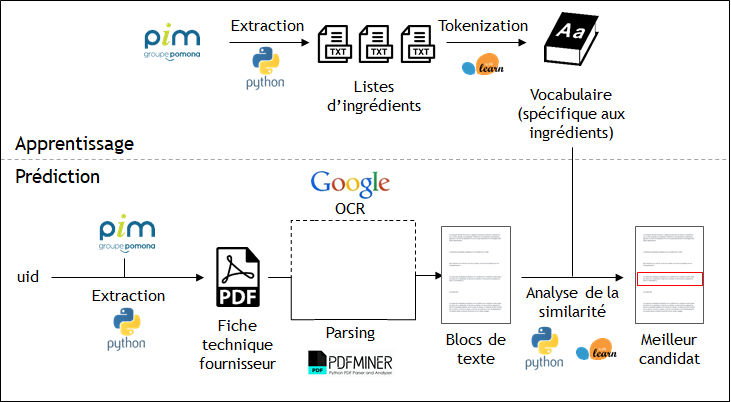
\includegraphics[width=0.9\linewidth]{img/open_model.png}
        \end{center}
        \caption{Schéma de principe du \og modèle ouvert \fg}
        \label{fig:open_model}
    \end{figure}     


        \section{Extraction des données}

        Ne garder que produits d'épicerie et boissons non alcoolisées

        \section{Conversion en blocs de texte}

        On utilise la bibliothèque PDFMiner.six. 
        Elle nous sort un long string qui contient le texte entier du document.
        On applique une \og bête \fg fonction : on splitte ce string quand on observe 2 retours à la lignes consécutifs.
        Le code est présenté en annexe.
        Pour le moment, vu la proportion importante de PDF dont le contenu est extractible

        \section{Train/Test split}

        On fait un split 50/50, on se base sur les uid pour identifier les produits.
        Sur le train set, on récupère les listes d'ingrédients du PIM.

        \section{Entrainement du modèle}

        L'entraînement est basique : on constitue seulement un vocabulaire en utilisant la fonctionnalité mise à disposition dans scikit-learn.

        \section{Calcul de la similarité}

        On calcule la similarité cosinus entre chacun des blocs, et le vocabulaire.
        On prend, systématiquement l'argmax de la similarité qu'on propose comme liste d'ingrédients.

        \section{Illustration des résultats obtenus}
    
        Mettre ici les résultats sur quelques fiches techniques présentées en annexe.
        Spoiler : rien que comme ça, les résultats sont encourageants.

        \section{Pistes d'améliorations identifiées}

        En plus de la mesure de la performance, qui est indispensable avant de pouvoir procéder à des ajustements.
        Pistes identifiées : 
        \begin{itemize}
            \item Faire un découpage du gros texte en blocs plus malin, potentiellement avec des expressions régulières
            \item Faire des \og ngrams de blocs \og, ce qui permettrait de parfois fusionner des blocs qui ont été séparés (car contenaient des retours à la ligne successifs)
            \item Essayer une autre manière de calculer la similarité ?
        \end{itemize}

    \chapter{Utilisation des données manuellement étiquetées}

    Comme présenté à la section\mref{ingredient_comparison} relative à la comparaison entre les données du PIM et celles récupérées lors de l'étiquetage, il y a un grand nombre d'écarts.
    Or, si on entraîne le modèle et qu'on mesure sa performance sur des données de mauvaise qualité, on aura de mauvais résultats.
    On va donc construire un modèle se basant sur les données manuellement étiquetées.
    Le fonctionnement de ce modèle est présentés à la \reffig{fig:ground_truth_model}.
    Le code utilisé à cette partie est présenté dans le notebook en annexe TODO ! METTRE UNE REFERENCE ICI.
    Les différents estimateurs spécifiques sont définis dans le module pimest TODO ! METTRE UNE REFERENCE ICI !
    
    \begin{figure}[htbp]
        \begin{center}
        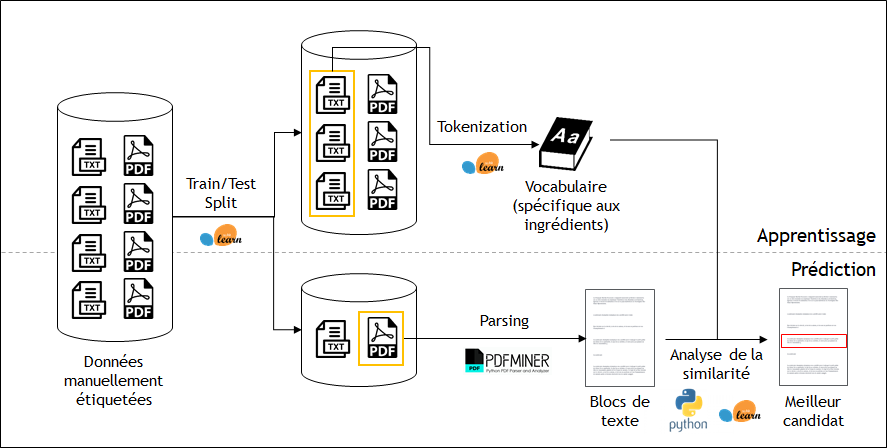
\includegraphics[width=0.9\linewidth]{img/ground_truth_model.png}
        \end{center}
        \caption{Schéma de principe du modèle basé sur les données étiquetées}
        \label{fig:ground_truth_model}
    \end{figure}     

        \section{Chargement des données manuellement étiquetées}

        La toute première étape est la constution d'un dataframe contenant : 
        \begin{itemize}
            \item les uid pour indexer les produits
            \item les listes d'ingrédients manuellement étiquetées depuis les fiches techniques
            \item le contenu de chacune des fiches techniques au format texte
        \end{itemize}
        On commence par charger les données du fichier csv contenant les uid et les listes d'ingrédients.
        Ensuite, un pipeline scikit learn d'acquisition des données est lancé.
        Il s'agit de 3 transformateurs en série, qui effectuent les travaux suivants :
        \begin{itemize}
            \item construction du chemin pointant vers les fiches techniques (sur la base des uid)
            \item construction d'une feature contenant les données des fichiers, en binaire
            \item construction du texte complet de la fiche technique (en se basant sur la library pdfminer.six)
        \end{itemize}
        Le résultat du lancement de ce pipeline est présenté à la \reftable{tbl:mod_GT_fulltexts}.

        {\renewcommand{\arraystretch}{1.5}%
        \begin{table}[htbp]
            \begin{center}
            {\scriptsize
            \begin{tabular}{p{\linewidth}}
\toprule
                                                                                                                                                                                                                                                                                                                                                                                                                                                                                                                                                                                                                                                                                                                                                                                                                                                                                                                                                                                                                                    text \\
\midrule
 NESCAFÉ® SPÉCIAL FILTRE\textbackslash n\textbackslash nDose individuelle de 2 g\textbackslash nTechnologie micro-grains\textbackslash n\textbackslash nCODE EAN (UC)\textbackslash n\textbackslash n3033710076017\textbackslash n\textbackslash nDENOMINATION LEGALE DU PRODUIT\textbackslash n\textbackslash nDESCRIPTION DU PRODUIT\textbackslash n\textbackslash nCafé instantané et café torréfié moulu.\textbackslash n\textbackslash nUne dominante Arabica pour l'arôme et une pointe de Robusta pour le \textbackslash ncorsé, associés à une torréfaction légère pour un café équilibré et peu \textbackslash namer.\textbackslash nSachet dose pour une tasse.\textbackslash n\textbackslash nDOSAGE PRECONISÉ\textbackslash n\textbackslash nMODE OPERATOIRE\textbackslash n\textbackslash nPour obtenir\textbackslash n\textbackslash n1 café Court (DA)\textbackslash n\textbackslash n1 café Long (DA)\textbackslash n\textbackslash nEau\textbackslash n\textbackslash n7\textbackslash n\textbackslash n12\textbackslash n\textbackslash ncl\textbackslash n\textbackslash ncl\textbackslash n\textbackslash nNESCAFÉ®\textbackslash n\textbackslash n SPÉCIAL FILTRE\textbackslash n\textbackslash n2\textbackslash n\textbackslash n2\textbackslash n\textbackslash ng\textbackslash n\textbackslash ng\textbackslash n\textbackslash nA reconstituer avec de l'eau. \textbackslash nTempérature de l'eau : 75°C\textbackslash nPour une qualité optimale, utilisez de l'eau filtrée.\textbackslash n\textbackslash nIngrédients : Café instantané, café torrefié moulu (3\%).\textbackslash n\textbackslash nINGRÉDIENTS\textbackslash n\textbackslash nPROFIL GUSTATIF\textbackslash n\textbackslash nIntensité\textbackslash n\textbackslash nConditionné sous atmosphère protectrice.\textbackslash n\textbackslash nENGAGEMENT QUALITÉ\textbackslash n\textbackslash n- NESTLÉ a un système de management de la qualité, le NMS (NESTLÉ \textbackslash nManagement System), en cohérence avec les systèmes ISO 9001 ... \\
 LENTILLES BLONDES 4mm\textbackslash n\textbackslash nRéférence PQG007-3.22.1\textbackslash nVersion\textbackslash nDate d'application :\textbackslash nPage 1/2\textbackslash n\textbackslash nG\textbackslash n\textbackslash n15/10/2019\textbackslash n\textbackslash nPrésentation\textbackslash n\textbackslash nCaractéristi -\textbackslash n\textbackslash nques \textbackslash n\textbackslash nphysico-\textbackslash nchimiques \textbackslash n\textbackslash nDéfinition\textbackslash n\textbackslash nOrigine\textbackslash nDénomination \textbackslash nlégale\textbackslash n\textbackslash nLentilles de couleur brun clair. Elles sont de forme biconvexe et \textbackslash npossèdent une peau assez épaisse. Leur diamètre est compris \textbackslash nentre 4mm et 5mm\textbackslash n\textbackslash nChine, Canada, France, Italie, USA, Turquie\textbackslash n\textbackslash nLentilles blondes\textbackslash n\textbackslash nProcess\textbackslash n\textbackslash nNettoyage, épierrage, triages\textbackslash n\textbackslash nConservation\textbackslash n\textbackslash n36 mois à l'abri de la chaleur et de l'humidité\textbackslash n\textbackslash nCritères d'analyses\textbackslash n\textbackslash nMoyenne/Tolérance\textbackslash n\textbackslash nMéthodes\textbackslash n\textbackslash nHumidité\textbackslash nMatières minérales étrangères\textbackslash nMatières végétales étrangères\textbackslash nGraines\textbackslash n\textbackslash nImpropres\textbackslash nBrisées\textbackslash nGermées\textbackslash n\textbackslash nCalibre 4-5 mm\textbackslash n\textbackslash n11,5\% / 16\%max\textbackslash n0,05\% / 1\%max\textbackslash n0,15\% / 0,5\%max\textbackslash n\textbackslash n0,5\% / 1\%max\textbackslash n0,4\% / 1\%max\textbackslash n0,05\% / 1\%max\textbackslash n95\% / 90\%min\textbackslash n\textbackslash nNF V03707\textbackslash n\textbackslash nMicrobiologie\textbackslash n\textbackslash nIl n'existe pas de réglementation concernant les exigences microbiologiques \textbackslash npour ce produit.\textbackslash n\textbackslash nPesticides\textbackslash nMét... \\
 FICHE TECHNIQUE \textbackslash n\textbackslash nPRODUIT FINI\textbackslash n\textbackslash n000100\textbackslash n\textbackslash nPurée de Poire Sans Sucres Ajoutés\textbackslash n\textbackslash nDate d'application: 05/05/2014\textbackslash n\textbackslash nPage: 1/2\textbackslash n\textbackslash nCoupelles Aluminium 120 x 95 g\textbackslash n\textbackslash nDéfinition\textbackslash n\textbackslash nCe produit est une purée de fruits obtenue à partir des parties comestibles des fruits (après broyage et sans \textbackslash nconcentration notable).\textbackslash nCe produit est sans sucres ajoutés: il contient uniquement les sucres naturellement présents dans les fruits.\textbackslash nLa purée présente une texture homogène et légèrement granuleuse.\textbackslash n\textbackslash nLa stabilité du produit est obtenue par pasteurisation et dosage à chaud.\textbackslash n\textbackslash nAspects nutritionnels\textbackslash n\textbackslash nDésignation et liste des ingrédients\textbackslash n\textbackslash nValeurs nutritionnelles (pour 100 g)\textbackslash n\textbackslash nDésignation légale :\textbackslash n\textbackslash nPurée de Poires sans sucres ajoutés *\textbackslash n* Contient les sucres naturellement présents dans \textbackslash nles fruits\textbackslash n\textbackslash nListe des ingrédients :\textbackslash n\textbackslash nPoire 99,9\%, antioxydant: acide ascorbique.\textbackslash n\textbackslash nMatières grasses\textbackslash n\textbackslash nEnergie\textbackslash n\textbackslash n65 kcal\textbackslash n\textbackslash n273 kJ\textbackslash n\textbackslash ndont acides gras saturés\textbackslash n\textbackslash nGlucides\textbackslash n\textbackslash nFibres alimentaires\textbackslash nPro... \\
\bottomrule
\end{tabular}

            }
            \caption{Exemples du contenu de fiches techniques au format texte (tronqués)}
            \label{tbl:mod_GT_fulltexts}
            \end{center}
        \end{table}
        }        

        \section{Découpage des textes en blocs}

        Le second travail est le découpage des textes en blocs. 
        Dans un premier temps, on va simplement effectuer ce découpage en splittant le texte lorsque deux retours à la ligne successifs sont détectés.
        Un exemple de découpage est présenté ci-dessous.

        \begin{multicols}{3}
        \begin{spacing}{1.0}
        {\tiny
        30/12/19 \newline -------------------------------------------------------------------- \newline Date d'impression :  \newline Remarque :  \newline Les informations contenues dans cette fiche technique sont données de bonne foi, en l’état actuel de nos connaissances, et selon  \newline les indications communiquées par le producteur ou le fournisseur. Il appartient au client de vérifier la conformité de la marchandise  \newline par rapport à l’usage qu’il en fait. \newline -------------------------------------------------------------------- \newline Création :  \newline -------------------------------------------------------------------- \newline 12/06/12 \newline -------------------------------------------------------------------- \newline 12 rue René Cassin \newline 37390 NOTRE DAME \newline -------------------------------------------------------------------- \newline Tél : \newline 02 47 85 55 00 \newline Fax :02 47 41 33 32 \newline -------------------------------------------------------------------- \newline FICHE TECHNIQUE \newline -------------------------------------------------------------------- \newline Mélange du trappeur, 70 g \newline Trapper blend, 70g \newline -------------------------------------------------------------------- \newline Code article KEREX \newline Nom latin (si disponible) \newline / EAN Code \newline Code barre  \newline -------------------------------------------------------------------- \newline / KEREX Code \newline -------------------------------------------------------------------- \newline / (Latin name) \newline -------------------------------------------------------------------- \newline TEEPTRAPPEUR \newline X \newline 3760063322262 \newline -------------------------------------------------------------------- \newline Poids net \newline Poids brut \newline Origine  \newline -------------------------------------------------------------------- \newline / net weight \newline / gross weight \newline / Origin \newline -------------------------------------------------------------------- \newline 0,07 Kilogramme \newline 0,125 Kilogramme \newline CANADA \newline -------------------------------------------------------------------- \newline / General information \newline -------------------------------------------------------------------- \newline Informations générales \newline DLUO conseillée / "Best before date" recommended \newline Nomenclature douanière / Customs code \newline Conditions idéales de stockage  \newline / Conditions of storage \newline Ingrédients :  \newline -------------------------------------------------------------------- \newline Conserver dans un endroit frais et sec \newline Store in a cool dry place \newline -------------------------------------------------------------------- \newline 5 ans / 5 years \newline 0910999900 \newline -------------------------------------------------------------------- \newline Sucre, poivre noir, coriandre, légumes déshydratés (ail, oignon, \newline poivron rouge), sel de mer, sucre d'érable, arôme d'érable naturel, \newline huile végétale (canola) \newline Sugar, black pepper, coriander, dehydrated vegetables (garlic, onion, \newline red bell pepper), sea salt, maple sugar, natural maple aroma, \newline vegetable oil (canola) \newline -------------------------------------------------------------------- \newline / Ingredients \newline -------------------------------------------------------------------- \newline Contaminants / Contaminating \newline Ionisation /  Irradation \newline -------------------------------------------------------------------- \newline OGM /  GMO \newline -------------------------------------------------------------------- \newline Pesticides/  Pesticides \newline -------------------------------------------------------------------- \newline Métaux Lourds \newline -------------------------------------------------------------------- \newline /  Heavy Metals \newline -------------------------------------------------------------------- \newline Allergènes et leurs dérivés (si présents) \newline /  Allergens (if existing) \newline -------------------------------------------------------------------- \newline Conformité à la directive 1999/2/CE (22/02/99)  \newline Produit non ionisé et ne contenant pas d’ingrédients ionisés.  \newline Not irradiated  \newline accordingly with the Reg 1999/2/CE (22/02/99). \newline Free from GMO \newline Ne contient pas d’OGM, est non soumis à l’étiquetage sur les OGM  \newline Conforme à la directive 396/2005 /CE  \newline In accordance with Reg 396/2005 /CE. \newline Conforme au règlement 1881/2006 /CE   \newline In accordance with Reg 1881/2006 /CE.. \newline -------------------------------------------------------------------- \newline Gluten \newline Crustacés \newline Oeufs \newline Poisson \newline Soja \newline Lait \newline Fruits à coque - Arachides \newline Céleri \newline Moutarde \newline Sésame \newline Sulfites \newline Lupin \newline Mollusques \newline -------------------------------------------------------------------- \newline / Gluten \newline / Crustaceans \newline / Eggs \newline / Fish \newline / Soy \newline / Milk \newline / Peanuts and Treenuts \newline / Celery and celeriac \newline / Mustarde \newline / Sésame \newline / Sulphites \newline / Lupin \newline / Shellfish \newline -------------------------------------------------------------------- \newline Absence \newline Absence \newline Absence \newline Absence \newline Absence \newline Absence \newline Absence \newline Absence \newline Absence \newline Absence \newline Absence \newline Absence \newline Absence \newline -------------------------------------------------------------------- \newline Caractères microbiologiques \newline -------------------------------------------------------------------- \newline / Microbiological characteristics \newline -------------------------------------------------------------------- \newline Microorganismes aérobies 30 °C \newline Escherichia coli  \newline Salmonelles \newline Levures \newline Moisissures \newline Aflatoxine Total \newline Aflatoxine B1 \newline -------------------------------------------------------------------- \newline / Total plat count (APC) \newline E. Coli \newline /   \newline / Salmonella \newline / Yeasts \newline / Moulds \newline / Total aflatoxin \newline B1 aflatoxin \newline /  \newline -------------------------------------------------------------------- \newline NF V05-051 < 6 000 000 / g \newline NF V08-053 < 10 / g \newline NF V08-052 Absence dans 25g \newline NF V08-059 < 10 000 / g \newline NF V08-059 < 10 000 / g \newline Kit Enzymatique < 10 ppb \newline Kit Enzymatique < 5 ppb \newline -------------------------------------------------------------------- \newline 
        }
        \end{spacing}
        \end{multicols}

        On constate que le découpage n'est pas idéal, cf. la fiche technique de ce produit, présentée en annexe \mref{ex:FT_meltrappeur}.
        Les séparations des cellules des tableaux de cette fiche ne sont pas prises en compte, et on a des blocs trop étendus.

        \section{Train/Test split}

        Dans la mesure où l'on possède assez peu de données, on va conserver un échantillon assez important dans le jeu d'entraînement : 400 produits (soit 80\% des données disponibles).

        \section{Entraînement du modèle}

        On fait tourner de la même manière que sur le modèle dit \og ouvert \fg

        \section{Illustration des prédictions obtenues}

        Un échantillon des prédictions obtenues est présenté dans la \reftable{tbl:GT_prediction_sample}.
        Pour éviter d'avoir des listes d'ingrédients prédites prenant trop de place dans cette table, celles dont la longueur dépasse 500 caractères ont été filtrées avant génération de cet échantillon.
        Les résultats présentés à cette table sont donc vraisemblablement biaisés, dans la mesure où les très longues listes prédites doivent avoir plus de chance d'être erronées.

        Les grandes tendances qui se dégagent à l'analyse de cette liste sont les suivantes : 
        \begin{itemize}
            \item globalement, les résultats sont bons. On retrouve régulièrement des morceaux de texte qui sont similaires à la liste cible
            \item une erreur qui revient régulièrement est le fait que le découpage en blocs est parfois imparfait, on sélectionne \og trop large \fg
            \item à l'inverse, le modèle n'a pas retiré des listes d'ingrédients prédites des mentions qui ont été rétirées lors de l'étiquetage manuel (cf. les règles d'annotation présentées en annexe \mref{annotation_rules}) : les préfixes de type \og Liste d'ingrédients : \fg, les allégations telles que \og Teneur totale en sucres : 60g pour 100g \fg \dots
            \item le modèle semble plus perfomant lorsque la liste d'ingrédients réelle est longue. On le vérifiera dans le chapitre relatif à la mesure de la performance du modèle
        \end{itemize}

        Un mot sur les cas où la liste d'ingrédients cible ou prédite sont vides :
        \begin{itemize}
            \item Les listes d'ingrédients cible sont vides lorsque la pièce jointe ne mentionnait pas de liste d'ingrédients. Cela peut arriver, et les produits concernés n'ont pas été sortis de l'échantillon. Il est 
            important de pouvoir aussi mesurer les faux positifs, qui sont nombreux avec cette techniques de choix systématique du meilleur candidat
            \item Les liste d'ingrédient prédites sont vides lorsque l'outil de parsing des pdf (pdfminer.six) n'a extrait aucun texte. C'est le cas quand la pièce jointe était un document imprimé qui a été scanné. Le texte n'est présent que sous forme d'image (cf. la fiche technique du sel en annexe \mref{ex:FT_sel})
        \end{itemize}

        {\renewcommand{\arraystretch}{1.5}%
        \begin{spacing}{1.0}
        \begin{center}
            {\scriptsize
            \begin{longtable}{p{7cm}p{7cm}}
\toprule
                                                                                                                                                                                                                                                                                            ingredients &                                                                                                                                                                                                                                                                                                  predicted \\
\midrule
\endhead
\midrule
\multicolumn{2}{r}{{Continued on next page}} \\
\midrule
\endfoot

\bottomrule
\endlastfoot
                                                                                                 sucre*, LAIT en poudre*, beurre de cacao*, pâte de cacao*, émulsifiant : lécithine de tournesol (E322), extrait de \newline vanille* \newline * matièrepremière issue de l'agriculture biologique \newline cacao : 27\% minimum &                                                                                            Liste des Ingrédients: \newline sucre*,  LAIT en poudre*,  beurre de cacao*,  pâte de cacao*,  émulsifiant : lécithine de tournesol (E322),  extrait de  \newline vanille* \newline * matièrepremière issue de l'agriculture biologique \\
                                                                                                                                                                                                                                                                                                      - &                                                                                                                                                                                                                                                                                                           \\
 Amidon de maïs* - Lait écrémé* - Sel - Fécule de pomme de terre* - Tomate* - Oignon* - Arômes naturels - Poivres* 3 \% (poivre vert*, poivre blanc*, poivre noir*) - Huile de tournesol* - Extrait de levure* - Sucre caramélisé* - Ail* - Maltodextrine de maïs*. \newline * issus de l’agriculture biologique &  Amidon de maïs* - Lait écrémé* - Sel - Fécule de pomme de terre* - Tomate* - Oignon* - Arômes naturels - Poivres* 3 \% (poivre vert*, poivre blanc*,  \newline poivre noir*) - Huile de tournesol* - Extrait de levure* - Sucre caramélisé* - Ail* - Maltodextrine de maïs*.  \newline * issus de l’agriculture biologique \\
                                                                                                                                                                                                                                                              semoule de blé dur supérieure et de l'eau &                                                                                                                                                                                                                                                    Ingrédients: semoule de blé dur supérieure et de l'eau  \\
                                                                                                                                                                                                                                                                                                      - &                                                                                                                           Boisson gazeuse aromatisée au jus de fruit à base de concentré \newline S.Pellegrino Orange 33 cl (Aranciata) \newline S.Pellegrino Citron 33 cl (Limonata) \newline Le plaisir des fruits à l’italienne \\
                                                                                                   Eau, maltodextrine, sel, arômes, sucre, arôme naturel de citronnelle, amidon modifié, ail en poudre, épices (combava, curcuma), extraits d'épices (gingembre, poivre), stabilisant (gomme xanthane). &                                                                                                  Eau, maltodextrine, sel, arômes, sucre, arôme naturel de citronnelle, amidon modifié, ail en poudre, épices (combava, curcuma), extraits  \newline d'épices (gingembre, poivre), stabilisant (gomme xanthane).    \\
                                                                                                                                                                                                     Sucre, cacao maigre en poudre (beurre de cacao : 11\% minimum), arôme vanille. \newline Cacao : 32\% minimum &                                                                                                                                                                                                                             Sucre, cacao maigre en poudre (beurre de cacao : 11\% minimum), arôme vanille.  \\
                                                                                                                                                                                  Sucre; sirop de glucose; graisse de palme; humectant: sirop de sorbitol; gélatine; acidifiant: acide citrique; arôme. &                                                                                                                                                                                                                                                                                                            \\
                                                                                                                                                                                                                     Gésier de dinde émincé 50\%, graisse de canard 47\%, sel, arômes naturels de poivre. &                                                                                                                                                                                                                    Gésier de dinde émincé 50\%,  graisse de canard 47\%, sel, arômes naturels de poivre.  \newline   \\
                                                                                                                                                                                                   Purée de tomates mi réduite (64\%), sucre, vinaigre, amidon modifié, sel, acidifiant : acide citrique &                                                                                                                                                                            Liste des ingrédients :  Purée de tomates mi réduite (64\%), sucre, vinaigre, amidon modifié, sel, acidifiant :  \newline acide citrique \\
\end{longtable}

            }
        \end{center}
        \end{spacing}
        }

        On illustre ici le résultat.

    \chapter{Mesure de la performance}
    
    Comme vu aux chapitre précédents, il est indispensable de mesurer la performance de nos modèles.
    On le fera sur le modèle se basant sur les données manuellement étiquetées.
    Le principe est présenté à la \reffig{fig:measured_model}.

    \begin{figure}[htbp]
        \begin{center}
        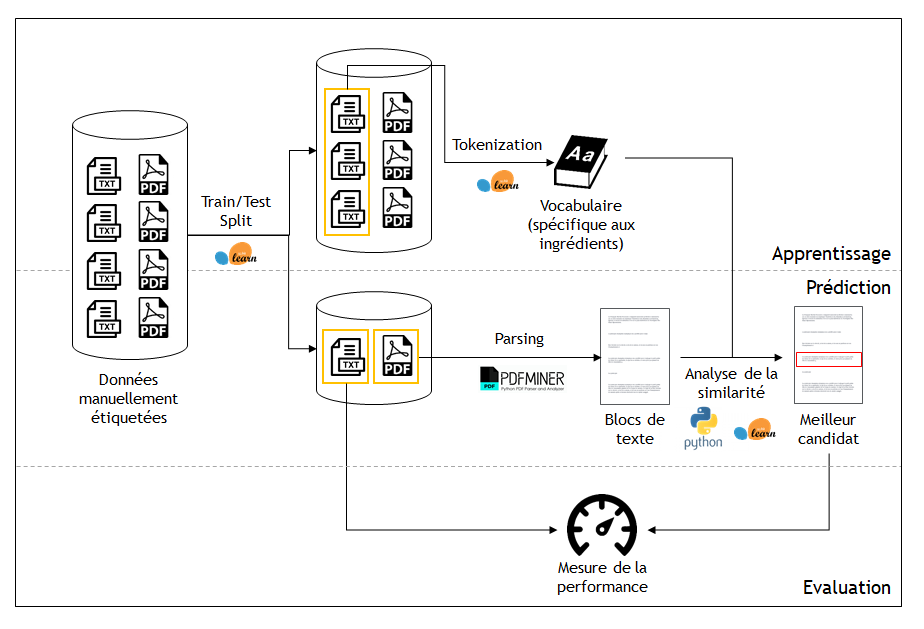
\includegraphics[width=0.9\linewidth]{img/measured_model.png}
        \end{center}
        \caption{Illustration de la méthodologie de mesure de la performance}
        \label{fig:measured_model}
    \end{figure}     

        \section{Précision}
        
        La métrique qui tombe le plus sous le sens est la précision.
        On mesure la proportion de prédictions qui sont égales à la ground truth.

            \subsection{Approche naïve}

            Illustration des résultats. 
            Comme on s'y attend, la précision sans transformation est très sévère.
            En particulier, prise en compte de la casse et des accents.
            La sortie du modèle contient des retours à la ligne à la fin des lignes de texte, là où la ground truth n'en contient pas.

            \subsection{Avec du \og text-postprocessing \fg}
        
            On assouplit un peu les contraintes en effectuant du text processing, à la fois sur la ground truth et les résultats du modèle.
            On tokenize (pour retirer ponctuation, \og blancs \fg), et on retire la casse et les accents pour constituer des textes qui ont plus de chance d'être égaux.
            Ce n'est pas une astuce pour améliorer les résultats, c'est juste que cette manière de mesurer est plus pertinente.
            Illustration des résultats en applicant diverses manières de \og post-processer \fg.

        \section{Fonctions de \og loss \fg spécifiques}

        On peut aussi définir des fonctions de loss, qui permettent d'être plus fin qu'une simple évaluation OK / KO du résultat du modèle.
        On calculera une distance entre le résultat du modèle, et de la ground truth.

            \subsection{Distance de Levenshtein}

            Brève description de chacune de ces distances.

            \subsection{Distance de Dameray-Levenshtein}

            Brève description de chacune de ces distances.
            
            \subsection{Distance de Jaro}
            Brève description de chacune de ces distances.

            \subsection{Distance de Jaro-Wrinkler}
            Brève description de chacune de ces distances.

            \subsection{Métriques non retenues}
            Distance de Hamming

            \subsection{Conclusion sur la métrique à utiliser}
            Une fois que cela aura été fait.


        \section{Cross-validation}
            
        On effectue une cross validation sur le modèle travaillant sur les données manuellement étiquetées.    
        
    \chapter{Transfer learning}
        
        \section{Principe du pré-entraînement}
        
        Expliquer qu'il s'agit d'une approche hybride des 2 modèles précédents
        On effectue une entraînement à la fois sur une partie des listes d'ingrédients du PIM, et sur une partie des données étiquetées.
        On vérifie ensuite, uniquement sur 

        \section{Illustration de l'impact sur la performance}

        Ici, on montre l'impact sur la performance, du fait d'intégrer des listes d'ingrédients.
        On met en abscisse le nombre de listes d'ingrédients qu'on ajoute, et en ordonnée la performance du modèle (avec barre d'erreurs, via cross validation).
        On regarde si l'effet est positif : cela montrera s'il est intéressant d'avoir plus de données.
        On regarde si on observe une saturation : cela montrera si on a déjà suffisamment de données sous formes de listes d'ingrédients dans le PIM, ou bien si ce serait intéressant d'en acquérir plus.

    \chapter{Hyperparameter tuning}
            
    On peut, dans l'optique d'améliorer la performance du modèle, ajuster certains paramètres et d'évaluer l'impact via une grid search.
    On fera tourner sur le modèle avec transfer learning.

        \section{Les paramètres ajustables}

            \subsection{La prise en compte des \og n-grams \fg dans la tokeinzation}

            On peut utiliser les n-grams lors de la tokenisation.

            \subsection{L'application de \og n-grams \fg de blocs}

            Voir si dans la recherche du meilleur candidat, on s'autorise la constitution de \og n-grams \fg de blocs.

            \subsection{L'utilisation d'expressions régulières dans le split des blocs}

            Voir si certaines expressions régulières pour splitter les blocs procurent de meilleurs résultats.

            \subsection{Applications d'autres fonctions de similarité}

            Voir l'impact d'utiliser d'autres manières de calculer la similarité.

            1 - autre chose que la similarité cosinus (fonction du nombre de mots du bloc et de la proportion de mots issus du vocabulaire des ingrédients)

            2 - en appliquant du TF et du TF-IDF

        \section{Application d'une grid search}

        Illustrer ici les résultats d'une grid search ou d'une random search si trop gourmand.